\documentclass[
    coverheight=9.249in,
    coverwidth=6.319in, % (pagesize - spinewidth) / 2
    spinewidth=1.8in,
    bleedwidth=0.306in,
    11pt,
    marklength=0pt,
  ]{bookcover}
  
  \usepackage{lettrine}
  \usepackage{fancybox}
  \usepackage{wrapfig}
  \usepackage[many]{tcolorbox}
  \usetikzlibrary{calc,positioning, shadings}
  \usepackage[T1]{fontenc}
  \usepackage{Alegreya} %% Option 'black' gives heavier bold face 
  
  \newcommand{\olpath}{../}
  \newcommand{\whitebg}[1]{%
  \tikz\node[circle,draw,minimum size=.9cm,
  fill=white,
  path picture={
      \node at (path picture bounding box){
          \includegraphics[width=.9cm]{\olpath#1}
      };
  }]{};
  }
  \newcommand{\bartosz}{
    \vspace{0pt}
    \begin{tcolorbox}[beamer,
      width=4cm,
      arc=0pt,
      boxsep=0pt,
      left=0pt,right=0pt,top=0pt,bottom=0pt,
      ] 
\includegraphics[width=4cm]{bartosz}
    \end{tcolorbox}
  }
  \newcommand{\OPTVersion}{0.0.0.0 - DO NOT USE}
  
  \definecolor{BackgroundColor}{HTML}{f3f6ed}
  \definecolor{SpineBackColor}{HTML}{262626}
  \definecolor{SpineFontColor}{RGB}{248,154,14}
  
  \begin{document}
  
  \begin{bookcover}
    \bookcovercomponent{color}{bg whole}{color=BackgroundColor}
    \bookcovercomponent{color}{spine}{color=SpineBackColor}
    \bookcovercomponent{normal}{front}{
    \vspace{2.5cm}
    \begin{center}
      \fontsize{40pt}{7em}\selectfont\bfseries
          CATEGORY THEORY \\FOR PROGRAMMERS
      \vfil
      \vspace*{1cm}
      
\includegraphics[width=.5\coverwidth]{piggie}
      \vfil
      \normalfont\Huge
      \hspace*{.8cm}\textbf{Bartosz Milewski}
      \vfil
      \vspace*{1cm}
    \end{center}}
    
    \bookcovercomponent{center}{spine}{
      \rotatebox[origin=c]{-90}{\color{SpineFontColor}\bfseries\Huge Category Theory for Programmers \hspace{2em} Bartosz Milewski}}
    
    \bookcovercomponent{normal}{back}{%
    \begin{minipage}[b][\coverheight][t]{\coverwidth}
      \begin{center}
        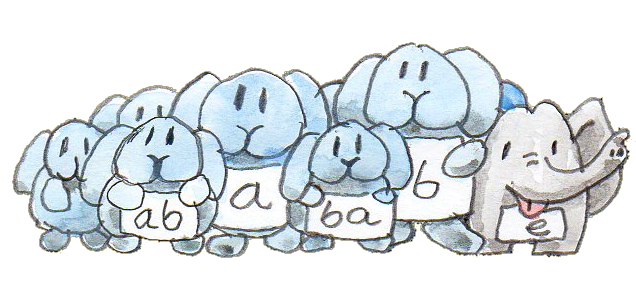
\includegraphics[width=.8\coverwidth]{bunnies}
        \begin{minipage}[t]{.8\coverwidth}
          % !TEX root = cover-blurb.tex
% Blurb on back cover

{
\fontsize{14}{17}\selectfont
\scshape{Category Theory}\normalfont\sffamily{}
is one of the most abstract branches of mathematics. It is usually taught to
graduate students after they have mastered several other branches of mathematics,
like algebra, topology, and group theory. It might, therefore, come as a shock that
the basic concepts of category theory can be explained in relatively simple terms
to anybody with some experience in programming. \\

That's because, just like programming,
category theory is about structure. Mathematicians discover structure in mathematical
theories, programmers discover structure in computer programs. Well-structured programs
are easier to understand and maintain and are less likely to contain bugs. Category theory
provides the language to talk about structure and learning it will make you
a better programmer.
\vfil

}

          \vspace{.5cm}
        \end{minipage}
        
        \begin{minipage}{.85\textwidth}
          \rule{\textwidth}{0.4pt}

          \begin{tabular}[h]{p{4cm} p{\textwidth}}
            \bartosz
            &
            \vspace{5pt}
            \begin{minipage}[b]{.55\coverwidth}
              \fontsize{11pt}{1.4em}\selectfont\textit{Category Theory for Programmers}
                is a compilation of blog posts by Bartosz Milewski, at bartoszmilewski.com.\\
                Edited by Igal Tabachnik. Licenced under CC BY-SA 4.0.
          \end{minipage}
        \end{tabular}
        \begin{flushright}
          \vspace{-2.5cm}
          \begin{minipage}[b]{4cm}
          \raggedleft
          \whitebg{fig/icons/by}
          \whitebg{fig/icons/cc}
          \whitebg{fig/icons/sa}
          \footnotesize{\texttt{\OPTversion}}
          \end{minipage}
        \end{flushright}
      \end{minipage}
    \end{center}
  \end{minipage}
  }
  \end{bookcover}
\end{document}